%\documentclass[11pt]{report}



%\begin{document}

\chapter{Quantum and Classical Oblivious Transfer}

Secure multiparty computation (SMC) has the potential to be a disruptive technology in the realm of data analysis and computation. It enables several parties to compute virtually any function while preserving the privacy of their inputs. However, most of its protocols’ security and efficiency relies on the security and efficiency of oblivious transfer (OT). For this reason, it is fundamental to understand the pros and cons of classical and quantum approaches. In this chapter, we start by analysing both the security and efficiency of classical OT protocols. Then, we compare these classical protocols with their quantum analog. However, we note that classical and quantum approaches use different information medium. Also, classical technology is indeed much more mature than quantum technology. These two observations make it dubious how to perform such a comparison. 

In chapter~\ref{chapter_QOT}, we reviewed several quantum OT protocols and, in particular, we explored BBCS-based QOT protocols. Beyond being resistant to quantum computer attacks, these protocols provide a practical way to perform OT within SMC. These are divided into two independent phases: oblivious key phase and transfer phase. The first phase corresponds to a precomputation phase that uses quantum technologies and is independent of the parties input elements ($m_0$, $m_1$ and $b$). The second phase only uses classical communication and is based on the precomputed elements from the first phase (oblivious keys). It can be argued that the precomputation phase is not so hungry-efficient as the transfer phase. This comes from the fact that the precomputation is independent of the parties' inputs and, thus, can be performed way before starting an SMC execution. Since the classical OT protocols can also be divided into these two phases, we can compare the transfer phase of both quantum and classical approaches. Furthermore, we do not need quantum equipment to be run concurrently witht he SMC execution.




\section{Classical Oblivious Transfer}


Let us start by presenting the Bellare-Micali (BM) OT protocol \cite{BM89} based on public key Diffie-Hellman. This exposition aims to shed some light on the issues related to classical OT implementations. The security and efficiency issues explored in this section also apply to most of the major classical protocols \cite{EGL85, NP01, CO15}.

We consider $\mathbb{G}_q$ to be a subgroup of $\mathbb{Z}^*_p$ with generator $g$ and order $q$, where $p$ is prime and $p = 2q + 1$. Also, we assume public knowledge on the value of some constant $C\in \mathbb{G}_q$. This constant guarantees that Bob follows the protocol. Also, for simplicity, we assume the protocol uses a random oracle described as a function $H$. For comparison purposes with quantum OT version presented in Chapter~\ref{chapter_QOT}, we split the BM OT protocol into two phases: precomputation phase and transfer phase. The first phase sets the necessary resources to execute the oblivious transfer in the second phase. The BM OT protocol $\Pi_{BM}$ is shown in Fig.~\ref{fig:BMOTProtocol}.


\begin{figure}[h!]
\centering
\begin{tcolorbox}[enhanced, 
                        frame hidden,
                        ]
                        
    \centerline{$\Pi_{BM}$ \textbf{protocol}}
            
    \
    
    \textbf{Alice's input:} $(m_0, m_1)\in\{0,1\}^l$ (two messages). 
    
    \textbf{Bob's input:} $b\in\{0,1\}$ (bit choice).
    
    \
    
    \textit{(Precomputation phase)}
    \begin{enumerate}
         \item Bob randomly generates $k\in \mathbb{Z}_q$ and computes $g^k$.
         \item Alice randomly generates $r_0, r_1\in \mathbb{Z}_q$ and computes $g^{r_0}$ and $g^{r_1}$.
    \end{enumerate}
    \textit{(Transfer phase)}
    \begin{enumerate}
    \setcounter{enumi}{2}
        \item Bob sets $\mathsf{pk}_b := g^k$. Also, he computes $\mathsf{pk}_{1-b} = C \cdot \mathsf{pk}_b^{-1}$.
        \item Bob sends both public keys $(\mathsf{pk}_0, \mathsf{pk}_1)$ to $S$.
        \item Alice checks if $(\mathsf{pk}_0, \mathsf{pk}_1)$ were correctly generated by computing their product: $C = \mathsf{pk}_0 \times \mathsf{pk}_1$.
        \item Alice computes and sends to Bob the two tuples: $E_0 = ( g^{r_0}, H(\mathsf{pk}_0^{r_0})\oplus m_0 )$ and $E_1 = ( g^{r_1}, H(\mathsf{pk}_1^{r_1})\oplus m_1 )$ for some hash function $H$.
        \item Bob is now able to compute $H(\mathsf{pk}_b^{r_b})$ and recover $m_b$.
    \end{enumerate} 
    
    \textbf{Alice's output:} $\bot$.
    
    \textbf{Bob's output:} $m_b$.
    
\end{tcolorbox} 
	\caption{Bellare-Micali classical OT protocol divided into two phases \cite{BM89}.}
	\label{fig:BMOTProtocol}
\end{figure}

\subsection{Security issues}

The Bellare-Micali OT protocol is secure if it complies with both the concealing and obliviousness property. The former is achieved because Bob does not send any information that reveals his input bit choice $b$ to Alice. The latter relies on Alice's ability to keep her randomly generated elements $r_0$ and $r_1$ private. Thus, the obliviousness property is compromised if Bob is able to compute the discrete logarithm of $g^{r_i}$ for $i=0,1$ (discrete logarithm problem).

The hardness of the discrete logarithm problem on cyclic groups is the basis of several other important protocols. Thus, it is crucial to understand its security limits. Nevertheless, it remains to be proven whether, given a general cyclic group $ \mathbb{G}_q$ with generator $g$ and order $q$, there exists a polynomial-time algorithm that computes $r$ from $g^r$, where $r\in \mathbb{Z}_q$. Indeed, the BM OT protocol's security relies on the assumption that Bob has limited computational power and is not able to compute the discrete logarithm of a general number.

Although the general discrete logarithm problem is not known to be tractable in polynomial-time, there are specific cases where it is possible to compute it efficiently. This leads to some classical attacks where the structure of the cyclic group considered is not robust enough. As an example, if a prime $p$ is randomly generated without ensuring that $p - 1$ contains a big prime $p_b$ in its decomposition, it is possible to use a divide-and-conquer technique \cite{PH78} along with some other methods (Shank's method \cite{S71}, Pollard's rho \cite{P78}, Pollard's lambda  \cite{P78}) to solve the discrete logarithm problem. In this case, the computation time will only depend on the size of $p_b$. So, the smaller the prime $p_b$, the faster the algorithm can be. In order to avoid these types of attacks, it is recommended to use safe primes, i.e. $p = 2q + 1$ prime where $q$ is also prime. However, it is computationally more expensive to find safe primes because they are less frequent when compared with prime numbers. Beyond the cyclic group structure, it is also important to find big enough prime numbers $p$. Otherwise, it is possible to compute the discrete logarithm in an acceptable time. As reported in \cite{ABDGGHHSTVVWZZ15}, after one week of precomputation, it is possible to compute the discrete logarithm in a 512-bit group in one minute by using the number field sieve algorithm. So, by following this method, after a week-long computation, Bob would be able to find both messages $m_0$ and $m_1$ of the BM OT protocol in one minute. In an SMC scenario based on the Yao approach \cite{Yao82}, where each OT performed corresponds to one input bit of Alice and the chosen group parameters are fixed, Bob would be able to get the keys corresponding to both $0$ and $1$ bit and, consequently, he would be able to discover all Alice's inputs. Therefore, at the expense of efficiency, it is necessary to use big enough prime numbers (2048-bit or larger), for which these classical attacks could not be feasibly implemented.

We have just seen specific examples where it is possible to break the security of OT protocol using classical techniques. However, it is known that it is possible to break the general discrete logarithm problem with a quantum computer. In 1995, Peter Shor published a quantum algorithm that is able to solve both prime factorization and discrete logarithm problems in polynomial-time \cite{Sho95}. This remarkable finding poses a threat to most of our currently deployed asymmetric cryptographic protocols (Rivest-Shamir-Adleman, elliptic-curve cryptography and Diffie-Hellman key exchange) as they have their security based on these computational assumptions. Therefore, in the BM OT protocol Bob would be able to perform two attacks with the help of a quantum computer:


\

\textbf{Quantum attack 1:}
\begin{enumerate}
    \item Bob computes the discrete logarithm of $g^{r_{1-b}}$ received from Alice using Shor's algorithm, i.e. $r_{1-b} = \log_g g^{r_{1-b}}$.
    \item Bob is then able to compute $H\big((g^{r_b})^k\big) = H(\mathsf{pk}_b^{r_b})$ and $H(\mathsf{pk}_{1-b}^{r_{1-b}})$ and get both messages $m_b$ and $m_{b-1}$.
\end{enumerate}

\textbf{Quantum attack 2:}
\begin{enumerate}
    \item Bob computes the discrete logarithm of $\mathsf{pk}_{1-b}$ with the Shor's algorithm, i.e. $s = \log_g \mathsf{pk}_{1-b}$.
    \item Bob is then able to compute $H\big((g^{r_b})^k\big) = H(\mathsf{pk}_b^{r_b})$ and $H\big((g^{r_{1-b}})^s\big) = H(\mathsf{pk}_{1-b}^{r_{1-b}})$ and get both messages $m_b$ and $m_{1-b}$.
\end{enumerate}

In the research literature, there are mainly two approaches to tackle this issue: the development of protocols with assumptions on the computational power of quantum computers or the development of protocols that make use of quantum technology. The former is known as post-quantum cryptography \cite{Bernstein2017} and its public-key cryptography protocols are generally more demanding due to the nature of the computational assumptions used. It is also worth stressing that these computational assumptions are still unproven and have survived just a few years of scrutiny, rendering it likely to be attacked in the near future. The latter is known as quantum cryptography \cite{Pirandola20}. It provides solutions without relying on asymmetric cryptography but it drastically increases the cost of technological equipment required. Finally, it is important to note that, in general, quantum protocols do not suffer from \textit{intercept now - decipher later} attack (everlasting security) because they base their security on quantum theory. On the contrary, this possible threat is always present in protocols based on computational assumptions.


\subsection{Efficiency issues}

In the previous section, we noted that every mitigation process used to increase security would bring a downside in efficiency: generating safe primes is more demanding, computing bigger exponents and module primes is heavier in general, and using post-quantum solutions require stronger computational assumptions and thus tends to increase the computational complexity. 

Now, let us understand the efficiency limitations of the BM OT protocol. We start by looking at the operations used in the protocol (random number generation, modular multiplication, modular inversion, modular exponentiation, hash function evaluation, XOR operation) from which the most demanding operation is modular exponentiation. For this reason, the complexity of BM OT heavily depends on the complexity of modular exponentiation. The number of modular exponentiations executed in each phase is summarised in the Table~\ref{table:BMOT_mexp}.


\begin{table}[h!]
\centering
\begin{tabular}{lcc}
\toprule
 & Alice & Bob \\
\midrule
\multicolumn{1}{l}{Precomputation phase}   & $2$  & $1$  \\
\multicolumn{1}{l}{Transfer phase} & $2$  & $1$\\
\bottomrule
\end{tabular}
\caption{Number of modular exponentiations in the BM protocol for each phase.}
\label{table:BMOT_mexp}
\end{table}

One of the most efficient methods to compute general modular exponentiation with $n-$bit numbers is through a square-and-multiply algorithm along with Karatsuba multiplication. The former method takes $\mathcal{O}(n)$ multiplications and the latter has complexity $\mathcal{O}(n^{1.58})$. Thus, the overall method takes $\mathcal{O}(n^{2.58})$ $n-$bit operations \cite{MVV01}. To set an overestimation on the OT generation rate, let us only consider the time (in CPU cycles) required to compute all modular exponentiation operations. We can use the following expression:

\begin{equation}
\label{eq:nOTs}
\Big( \frac{C_{mexp}}{C_{cycles}} \times N_{mexp} \Big)^{-1}
\end{equation}
where $C_{mexp}$ is the number of CPU cycles required to compute one modular exponentiation, $C_{cycles}$ is the CPU frequency (number of cycles per second) and $N_{mexp}$ is the number of modular exponentiations performed in the OT implementation. This expression only renders an overestimation because it depends on both the implementation of the modular exponentiation operation and the CPU frequency used. 

Considering a standard CPU operating around $2.5$ GHz ($C_{cycles} = 2.5\times 10^9 $ cycles per second) and a very efficient implementation of modular exponentiation \cite{G11} ($C_{mexp} \sim 400\,000$ CPU cycles), the BM OT protocol would be able to perform at most $\sim 1041$ BM OTs in one second as represented in Fig.~\ref{fig:nOTsplot}.
\begin{figure}[]
\centering
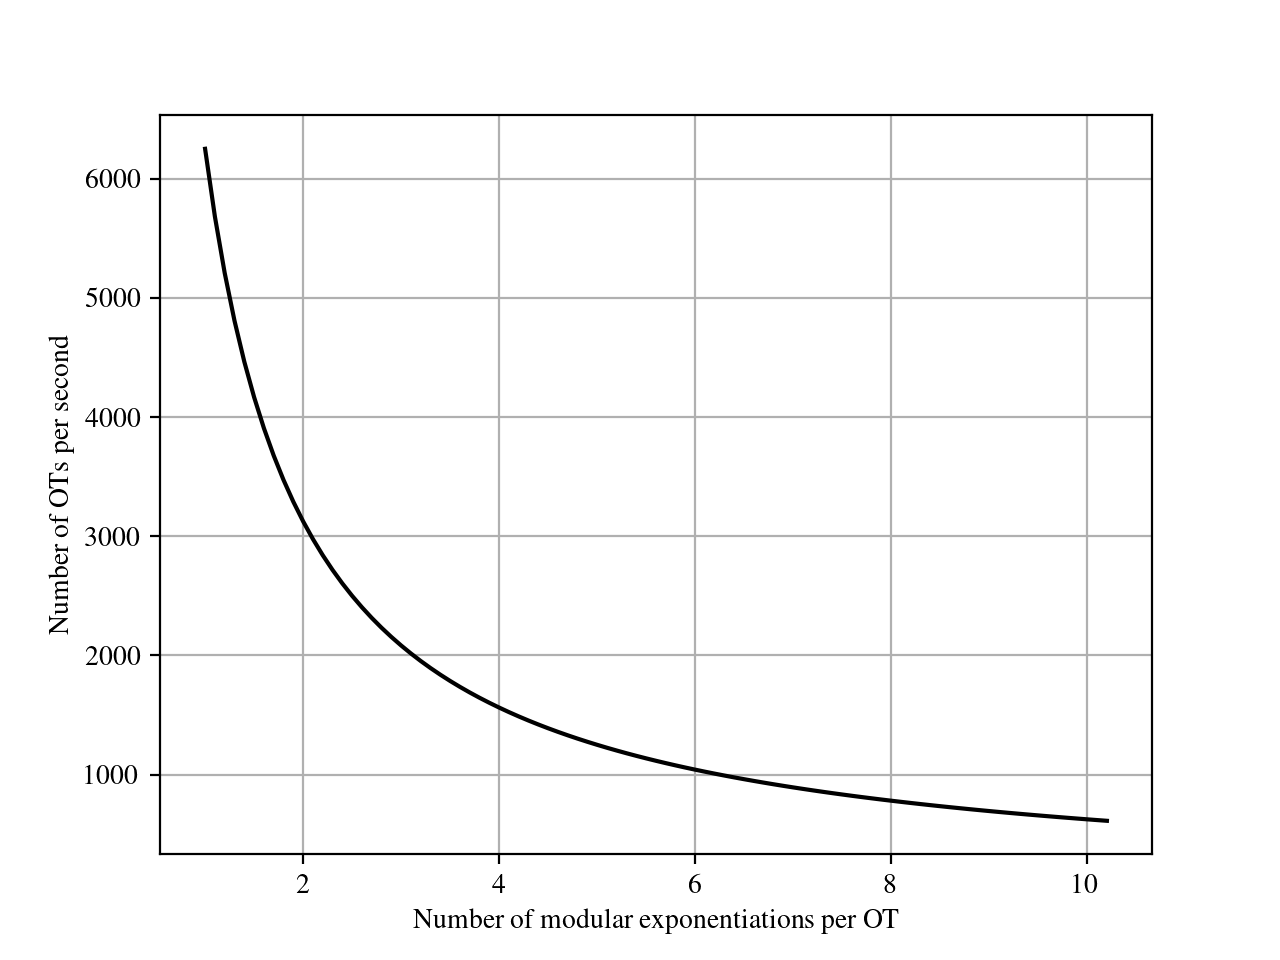
\includegraphics[width=0.8\textwidth]{Chapter_QuantumAndClassicalObliviousTransfer/nOTperSeccond.png}
\caption{Plot of expression (\ref{eq:nOTs}) on the overestimation of OT rate against the number of modular exponentiation operations required per OT.}
\label{fig:nOTsplot}
\end{figure}
Note that this is a very loose overestimation on the number of OT per second. Here, we just took into consideration the computational complexity of modular exponentiation and we assumed that all the other operations do not have a big impact on the computation time. So, we can conclude that the real OT rate must be well below this threshold. In fact, as reported in \cite{ALSZ13}, it takes around $18$ ms to generate a similar OT protocol: Naor-Pinkas OT \cite{NP01}, which requires $5$ modular exponentiations. This corresponds to a rate of just $56$ OT per second.

The OT rates presented above lead to serious constraints on the execution of SMC protocols that rely on OT. The Yao SMC protocol \cite{Yao82} uses boolean circuits to privately compute the desired functionality and requires as many OT as half the number of input wires. Thus, the execution time of the OT phase of the Yao protocol with a $32\, 000$ input boolean circuit would take at least $16$ seconds using our rough  OT rate estimation and around $2$m$23$s using Naor-Pinkas OT rate. In a deployment environment where it is required to evaluate several rounds of the same circuit, this approach turns out to be impractical and higher rates must be achieved.

\subsection{OT extension protocols} \label{Ext-OT}

Since most of the required computation to achieve OT comes from asymmetric cryptographic primitives that use modular exponentiation, it would be desirable to substitute it by more efficient methods. Symmetric cryptography has the advantage to be more efficient than asymmetric cryptography. Also, the known quantum attacks based on the Grover's algorithm only provide a quadratic advantage over classical approaches, which can be mitigated by doubling the size of the symmetric keys \cite{Bernstein2017}. Unfortunately, it was proved by Impagliazzo and Rudich that OT protocols require asymmetric cryptographic assumptions \cite{IR99}. This means OT cannot be performed by symmetric cryptographic tools alone.

Nonetheless, researchers developed some OT schemes to circumvent Impagliazzo and Rudich result by means of hybrid protocols, mixing symmetric and asymmetric cryptography. This idea was introduced by Beaver \cite{B96}, where he showed that it is possible to extend the number of OT using symmetric cryptography when a small number of base OT is created using asymmetric cryptography. Although Beaver's protocol was very inefficient, it paved the way to more efficient implementations \cite{IKNP03, N07, NNOB12, ALSZ13, ALSZ15}. Currently, one of the most efficient protocols is able to generate around 10 million OTs in 2.62 seconds in a back-to-back scenario \cite{ALSZ13}. Since these protocols use a small number of base OT and quantum secure symmetric tools, the security of the extended protocol is mainly dependent on the security of the base OT protocol. Moreover, the protocol that we analyse in section~\ref{Ext-OT_comp} \cite{ALSZ13} is not secure against malicious parties and must only be deployed in a semi-honest environment. Protocols that are secure against malicious parties need an extra consistency check phase which increases their complexity \cite{ALSZ15, KOS15}.


\section{Oblivious Transfer complexity analysis} \label{HQOT_comp}

In this section, we compare the complexity of the optimized O-OT version of HQOT presented before and well known classical protocols. The O-OT protocol is divided into two phases: the oblivious key distribution phase (we also call it a \textit{precomputation} phase) and the transfer phase. The first phase of O-OT is similar to the HQOT oblivious key phase \cite{Lemus20} presented in section \ref{HQOT} but the second phase follows the protocol shown in section \ref{O-OT}. In order to fairly compare the O-OT protocol with other protocols, we have to divide them in these two phases. We apply the following rule: all the steps used in the protocol that are independent of the messages ($m_0$ and $m_1$) and of the bit choice ($b$) are considered to be part of the precomputation phase, otherwise they are included in the transfer phase. Since the precomputation phase can be implemented before the execution of the Yao GC protocol, it is more important to guarantee that the transfer phase has small complexity. Furthermore, here we will only compare the complexity among the different protocols' transfer phase because their precomputation phase rely on different technologies. Since quantum technologies are still in their infancy and constantly evolving, it is difficult to compare the efficiency with classical approaches. Nevertheless, it is worth stressing that the oblivious key phase of O-OT protocol is linear in all its security parameters. In fact, as presented in \cite{Lemus20}, its time complexity is of order $\mathcal{O}(k(2l + t))$, where $k$ is the security parameter of the hash-based commitments, $2l$ is the number of qubits sent used to directly generate the oblivious keys and $t$ is the number of testing qubits.

\subsection{Classical OT} \label{C-OT_comp}

In section \ref{Classical-OT} we divided the well known Bellare-Micali protocol in these two phases and concluded that it requires three exponentiations during the transfer phase. In Table~\ref{table:ClassicalOT_comparison} we present the number of required modular exponentiations and communication rounds during the transfer phase of four well known classical protocols that have their security based on the computational hardness of the Discrete Logarithm problem. 

%\begin{table}[!b]
%\processtable{Number of modular exponentiation operations and communication rounds executed during the transfer phase of several classical protocols.\label{table:ClassicalOT_comparison}}
%{\begin{tabular*}{20pc}{@{\extracolsep{\fill}}lcc@{}}\toprule
%Protocol & Exponentiation & Comm. rounds \\
%\midrule
%EGL \cite{EGL85}      & $3$              & $2$\\ 
%BM  \cite{BM89}     & $3$              & $2$ \\ 
%NP  \cite{NP01}     & $2$             & $2$  \\ 
%SimpleOT \cite{CO15} & $1$              & $2$           \\
%\botrule
%\end{tabular*}}{}
%\end{table}

From the Table~\ref{table:ClassicalOT_comparison} we see that the most efficient protocol (SimpleOT \cite{CO15}) still requires one exponentiation operations and $2$ communication rounds. From the above formula (\ref{eq:nOTs}) and setting $C_{mcyles} = 2.5 \times 10^9$, $C_{mexp} = 400\,000$ and $N_{mexp} = 1$, we get an overestimation of around $6 000$ OT per second. Comparing with the rate achieved by OT extension protocols ($10$ million OT in $2.62$), it is still very inefficient. Also, note that the number of modular exponentiations do not decrease in their random versions. 

This means that the current classical OT protocols have a computational complexity limited by $\mathcal{O}(n^{2.58})$ bit operations due to modular exponentiation. The O-OT protocols only depends on simple bit operations (XOR, truncation and comparison), meaning its computational complexity is linear in the length of the messages $\mathcal{O}(n)$.

Also, it is important to stress that none of the above protocols are secure against quantum computer attacks. In order to have classical OT protocols with this level of security, we need to follow Post-Quantum approaches which may lead to more demanding operations \cite{PST19}. As reported in \cite{MR19}, using Module Learning With Errors (MLWE) based Kyber key encapsulation \cite{CrystalKyber17}, it takes 24 ms to generate one Oblivious Transfer in a LAN network. This leads to a rate of just 41 OT per second which is even lower than the rate reported by \cite{ALSZ13} for the Naor-Pinkas \cite{NP01}: 56 OT per second. In \cite{NTRUOT1, NTRUOT2}, the authors present a 1-out-of-$n$ OT based on the NTRU post-quantum encryption system \cite{NTRU} and compare it with the SimpleOT \cite{CO15} version. In this case, although the sender and receiver phases are more efficient individually, the overall NTRU OT protocol is still less efficient. For the highest security level, it takes around $1.372$ ms to generate one OT with the post-quantum approach, whereas it takes $0.727$ ms using the original SimpleOT protocol. These timings lead to the rates of $728$ and $1375$ OT per second, respectively. It is important to note that these protocols are still prone to \textit{intercept now - decipher later} attacks since they are based on computational assumptions that are only \textit{believed} (and not proved) to be secure against quantum computer attacks.


\subsection{OT extension} \label{Ext-OT_comp}

\begin{figure}[!t]
\centering
\framebox[\linewidth][l]{%
    \parbox{0.95\linewidth}{%
    \begin{center}
        \textbf{General OT extensions protocol}
    \end{center}
    
    \textbf{Sender input:} $m$ pairs $(x^0_j, x^1_j),\, \forall 1\leq j\leq m$ of $l$-bit strings.
    
    \textbf{Receiver input:} $m$ selection bits $\textbf{r} = (r_1, ..., r_m)$.
    
    \
    
    \textit{Initial OT phase (Precomputation phase)}
    \begin{enumerate}
         \item $S$ randomly generates a string $\textbf{s} = (s_1, ..., s_\kappa)$.
         \item $R$ randomly chooses $\kappa$ pairs of $\kappa$-bit strings $\{(\textbf{k}^0_i, \textbf{k}^1_i)\}^\kappa_{i=1}$.
         \item $R$ and $S$ execute $\kappa$ base OTs, where $S$ plays the role of the receiver with input $\textbf{s}$ and $R$ plays the role of the sender with messages $(\textbf{k}^0_i, \textbf{k}^1_i)\, \forall 1\leq i\leq \kappa$.
    \end{enumerate}
    \textit{OT extension phase (Transfer phase)}
    \begin{enumerate}
    \setcounter{enumi}{3}
        \item $R$ applies a pseudorandom number generator $G$ to $\textbf{k}^0_i$, i.e. $\textbf{t}^i = G(\textbf{k}^0_i)$. Computes $\textbf{u}^i = \textbf{t}^i \oplus G(\textbf{k}^1_i) \oplus \textbf{r}$ and sends $\textbf{u}^i$ to $S$ for every $1\leq i\leq \kappa$.
        \item $S$ computes $\textbf{q}^i = (s_i \cdot \textbf{u}^i) \oplus G(\textbf{k}^{s_i}_i)$.
        \item $S$ sends $(y^0_j, y^1_j)$ for every $1\leq j\leq m$, where $y^0_j = x^0_j\oplus H(j,\textbf{q}_j)$, $y^1_j = x^1_j\oplus H(j,\textbf{q}_j\oplus \textbf{s})$ and $\textbf{q}_j$ is the $j$-th row of the matrix $Q = [ \textbf{q}^1 | ...| \textbf{q}^\kappa]$. Note that, in practice, it is required to transpose $Q$ to access its $j$-th row.
        \item $R$ computes $x^{r_j}_j = y^{r_j}_j \oplus H(j, \textbf{t}_j)$.
    \end{enumerate} 
    
    \textbf{Sender output:} $\bot$.
    
    \textbf{Receiver output:} $(x^{r_1}_1, ..., x^{r_m}_m)$.
    }%
}
\caption{Precomputation and transfer phases of OT extensions protocol presented in \cite{ALSZ13}.}
\label{fig:ALSZ13Protocol}
\end{figure}

%\begin{table}[!b]
%\processtable{Computational complexity comparison between ALSZ13 \cite{ALSZ13} OT extension protocol and O-OT from section \ref{O-OT}.\label{table:CvsQ_OT_comparison_computation}}
%{\begin{tabular*}{20pc}{@{\extracolsep{\fill}}lcc@{}}\toprule
%Operation & ALSZ13 & O-OT \\
%\midrule
%PRG (AES)     & $3\kappa$              & -\\ 
%Hash (SHA-1)    & $3m$              & - \\ 
%Bitwise XOR      & $3\kappa m + \textcolor{red}{3ml} + \kappa$             & $\textcolor{red}{3ml} $  \\ 
%Bitwise AND  & $\kappa m$              & -           \\
%Matrix Transposition & $m\log m$              & -           \\
%Bitwise comparison & -             & $2ml$           \\
%Bitwise truncation & -            & $3ml$           \\
%\botrule
%\end{tabular*}}{}
%\end{table}

%\begin{table}[!b]
%\processtable{Communication complexity comparison between ALSZ13 \cite{ALSZ13} OT extension protocol and O-OT from section \ref{O-OT}.\label{table:CvsQ_OT_comparison_communication}}
%{\begin{tabular*}{20pc}{@{\extracolsep{\fill}}lcc@{}}\toprule
% & ALSZ13 & O-OT \\
%\midrule
%Bits sent     & $\textcolor{red}{2ml}  + m\kappa$              & $\textcolor{red}{2ml} + ml $\\ 
%\botrule
%\end{tabular*}}{}
%\end{table}

As we explained in section \ref{Ext-OT}, several techniques based on an hybrid symmetric-asymmetric approach were developed as a way to increase the OT execution rate. These techniques use a small number $\kappa$ ($=128$) of base OT protocols and extend this resource to $m$ ($=10\,000\,000$) OT executions, where $ m >> \kappa$. 

Again, in order to compare the OT extension approach with the O-OT, the OT extension protocols must be decomposed into two phases: precomputation phase and transfer phase. Here we make a bit-wise comparison of the communication and computational complexity of $m$ O-OT and one OT extension because OT extension protocols execute a predetermined number ($m$) of OTs at once.

Let us consider the OT extension protocol proposed in \cite{ALSZ13} (ALSZ13), which, at the time of writing, reports the fastest implementation: 10 million OT in 2.68 seconds. This protocol is originally divided into two phases: initial OT phase and OT extension phase. Note that these two phases correspond exactly to our division of precomputation and transfer phases. Thus, for comparative purposes, we are only interested in the second phase. In Tables~\ref{table:CvsQ_OT_comparison_computation} and~\ref{table:CvsQ_OT_comparison_communication}, we show the computational and communication complexity of both protocols, respectively.

In the Table~\ref{table:CvsQ_OT_comparison_computation}, PRG stands for Pseudorandom Generator, $\kappa$ represents the number of base OTs executed in the OT extension precomputation phase, $m$ is the number of final OTs and $l$ is the length of the OT strings. Also, we consider that $l \sim \kappa$ have the same order of magnitude, meaning they represent the same cost of bits. This is so, because $\kappa = 128$ in \cite{ALSZ13} and the key length used in the garbled circuits are $l = 128, 192$ or $256$. The red colored text in the table represents the operations omitted in a sender randomized version. So, we easily see that the Sender Random OT extension protocol do not gain any advantage over the SR-OT because they correspond to the same reduction in the number of bit operation and communication.

We have that the communication complexity is exactly the same in both protocols: $\sim 3ml$. So, the OT extension does not have any advantage over O-OT during the communication phase. Regarding their computational complexity, we have to compare the cost of $ml$ bit operations in O-OT against $3\kappa$ AES, $3m$ SHA-1 and $\kappa + m\log m$ bit operations in ALZS13 OT extension. 

Firstly, we can conclude that O-OT transfer phase is asymptotically more efficient than OT extension transfer phase. The computational complexity of OT extension is not linear in the number of OT executions, $\mathcal{O}(m\log m)$, whereas it is linear in the case of O-OT, $\mathcal{O}(m)$. Thus, for a bounded value $l$, $m\log m > ml$ asymptotically. However, in practice, for $l \sim 128$, it would take around $m>10^{50}$ Oblivious Transfers to actually have $m\log m > ml$. Secondly, when comparing $ml$ bit operations with $3m$ SHA$-1$ computations, we conclude that O-OT uses less bit operations. Each execution of SHA$-1$ \cite{NISTSHA} requires 80 rounds of several bit operations. If we underestimate the cost of each round and we assume it only requires two bit operations, we get that ALSZ13 OT extension protocol requires at least $3 \times 80\times 2 m = 480 m > ml, \, \forall m$. 

%Let us plot in Fig.~\ref{fig:CvsQ_OT_comparison} the number of bit operations for both protocols. In the case of ALSZ13 OT extension, we underestimate the number of bit operations by considering that SHA$-1$ only costs $480m$ bit operations and that PRG (AES) does not involve any cost. 

%\begin{figure}[!t]
%\centering
%\includegraphics[width=0.5\textwidth]{O-OTVsEXT_OT.png}
%\caption{Bit operation comparison between the transfer phase of O-OT and Extension %OT protocols.}
%\label{fig:CvsQ_OT_comparison}
%\end{figure}

From this, we conclude that O-OT transfer phase competes with the ALSZ13 corresponding phase and has the potential to be more efficient. It is important to stress that O-OT efficiency performance of the transfer phase comes along with a drastic increase in the security of the protocol: while ALSZ13 protocol relies on computational assumptions of the base OT, O-OT is proved to be secure against quantum computers; while ALSZ13 is a semi-honest protocol (assumes well-behaved parties that follow the protocol), O-OT is secure against any corrupted party. Indeed, in order to get a fair comparison, we should consider OT extension protocols that are secure against malicious parties. The work developed in \cite{IKNP03} presented for the first time a protocol in the malicious scenario, which was latter optimized by KOS15 \cite{KOS15} and ALSZ15 \cite{ALSZ15}. Both optimizations carry out one run of the semi-honest OT extension presented in ALSZ13 plus some consistency checks. The protocol presented in \cite{KOS15} adds to ALSZ13 a \textit{check correlation} phase after the transfer phase and the protocol presented in \cite{ALSZ15} adds a \textit{consistency check} phase during the transfer phase. This means that both malicious protocols' transfer phases have greater computational and communication complexity when compared with ALSZ13. Therefore, we can easily deduce that O-OT transfer phase has less computational and communication complexity than its classical equivalents with respect to the adversary model used.


\subsection{Oblivious Transfer comparison}

To implement practical SMC protocols, we need to be able to execute OT with a rate of the order of millions of OT per second. To reach this rate, classical solutions make use of extension algorithms: generate a small number $\kappa$ of base OT (precomputation phase as in HQOT) and extend them to $m$ ($\kappa << m$) real OT through symmetric cryptography \cite{IKNP03} (oblivious transfer phase). Currently, the most efficient OT extension protocols developed in the semi-honest model is reported by \cite{ALSZ13} (ALSZ13) and in the malicious model it is reported by \cite{K15} (KOS15). In \cite{Santos2021}, the authors showed that the overall complexity in the transfer phase of ALSZ13 is bigger than that of HQOT. Furthermore, they argued that KOS15 complexity is also bigger than HQOT but do not perform a complexity comparison between them. Here, we analyse the complexity of the KOS15 protocol which is implemented in the Libscapi library and we compare it with HQOT.

\subsubsection{KOS15 and HQOT comparison}

KOS15 protocol is very similar to ALSZ13 with the addition of a \textit{check correlation} phase. This phase ensures that the receiver is well behaved and does not cheat. The KOS15 protocol that generates $m$ $l$-bit string OT out of $\kappa$ base OT with computational security given by $\kappa$ and statistical security given by $w$ is shown in Figure~\ref{fig:K15Protocol}. Note that in Figure~\ref{fig:K15Protocol} we join all the subprotocols presented in the original paper: $\prod^{\kappa, m'}_{\textsc{COTe}}$, $\prod^{\kappa, m}_{\textsc{ROT}}$ and $\prod^{\kappa, m}_{\textsc{DeROT}}$. Also, they identify $\mathbb{Z}^\kappa_2$ with the finite field $\mathbb{Z}_{2^\kappa}$ and use $``\cdot"$ for multiplication in $\mathbb{Z}_{2^\kappa}$. For example, the element $\boldsymbol{t}_j$ in $\sum_{j=1}^{m'} \boldsymbol{t}_j \cdot \chi_j$ (Figure~\ref{fig:K15Protocol}, step $10$) should be considered in $\mathbb{Z}_{2^\kappa}$.

Similarly to HQOT, the KOS15 starts with a precomputation phase that can be carried out before the actual computation of the OT protocols. However, in the HQOT, the precomputation phase is based on quantum technologies while the transfer phase is solely based on classical methods. Since it is not clear how to compare quantum and classical protocols, we only focus our comparison on the transfer phase of both protocols. 

Note that in the original KOS15 paper \cite{K15} the computation of pseudorandom generator $G$ is carried out in the OT extension phase. However, these $3\kappa$ $G$ computations can be executed during the precomputation phase because they do not depend on the input elements. As mentioned before, the additional steps that KOS15 added to the ALSZ13 protocol are steps $9-11$ (check correlation phase). Here, both parties start by calling a random oracle functionality $\mathcal{F}_{\text{Rand}}(\mathbb{F}^{m'}_{2^\kappa})$ that provides them with equal random values. The receiver has to compute twice $m'$ $\kappa$-bit sums, $m'$ $\kappa$-bit multiplication and sends $2\kappa$ bit ($x$ and $t$) to the sender. Finally, the sender has to compute $m'$ $\kappa$-bit sums and $m'$ $\kappa$-bit multiplication. We consider karatsuba method for multiplication with complexity $O(\kappa^{1.585})$ and schoolbook addition with complexity $O(\kappa)$. Therefore, we consider that the sum of two $\kappa$ takes $\kappa$ bit operations and the multiplication takes $\kappa^{1.585}$.

%Parameters of OTe:

%Dizer que juntamos todas as funcionalidades descritas no paper: dizer quais são (sem explicar)

%Explicar a associaçao de $F^k_2$ e $F_2^k$ e referir operações.

\begin{figure}[!t]
\centering
\framebox[\linewidth][l]{%
    \parbox{0.95\linewidth}{%
    \begin{center}
        \textbf{General OT extensions protocol \cite{K15}}
    \end{center}
    
    \textbf{Sender input:} $m$ pairs $(x^0_j, x^1_j),\, \forall 1\leq j\leq m$ of $l$-bit strings.
    
    \textbf{Receiver input:} $m$ selection bits $\boldsymbol{r} = (r_1, ..., r_m)$.
    
    Let $m' = m + (\kappa + w)$.
    
    \
    
    \textit{Initial OT phase (Precomputation phase)}
    \begin{enumerate}
         \item $S$ randomly generates a string $\boldsymbol{s} = (s_1, ..., s_\kappa)$.
         \item $R$ randomly chooses $\kappa$ pairs of $\kappa$-bit strings $\{(\boldsymbol{k}^0_i, \boldsymbol{k}^1_i)\}^\kappa_{i=1}$.
         \item $R$ and $S$ execute $\kappa$ base OTs, where $S$ plays the role of the receiver with input $\boldsymbol{s}$ and $R$ plays the role of the sender with messages $(\boldsymbol{k}^0_i, \boldsymbol{k}^1_i)\, \forall 1\leq i\leq \kappa$.
         \item $R$ applies a pseudorandom number generator $G$ to $\boldsymbol{k}^0_i$ and $\boldsymbol{k}^1_i$: $\boldsymbol{t}^i = G(\boldsymbol{k}^0_i)$ and $\boldsymbol{t}^i_1 = G(\boldsymbol{k}^1_i)$. Also, set $\boldsymbol{T}^i = \boldsymbol{t}^i \oplus \boldsymbol{t}^i_1$.
         \item $S$ applies $G$ to $\boldsymbol{k}^{s_i}_i$ and sets $\boldsymbol{g}^{s_i}_i = G(\boldsymbol{k}^{s_i}_i)$.
    \end{enumerate}
    \textit{OT extension phase (Transfer phase)}
    
    \textit{\hspace{0.25cm} Extend}
    \begin{enumerate}
    \setcounter{enumi}{5}
        \item $R$ generates random elements $r_j$, for $r\in [m+1, m']$ and resize $\boldsymbol{r} = (r_1, ..., r_m, r_{m+1}, ..., r_{m'})$.
        \item $R$ computes $\boldsymbol{u}^i = \boldsymbol{T}^i \oplus \boldsymbol{r}$ and sends $\boldsymbol{u}^i$ to $S$ for every $1\leq i\leq \kappa$.
        \item $S$ computes $\boldsymbol{q}^i = (s_i \times \boldsymbol{u}^i) \oplus \boldsymbol{g}^{s_i}_i$ for every $1\leq i\leq \kappa$.
    \end{enumerate}
    \textit{\hspace{0.25cm} Check correlation}
    \begin{enumerate}
    \setcounter{enumi}{8}
        \item Sample $(\chi_1, ..., \chi_{m'})\leftarrow \mathcal{F}_{\text{Rand}}(\mathbb{F}^{m'}_{2^\kappa})$.
        \item $R$ computes $x = \sum_{j=1}^{m'} r_j \cdot \chi_j$ and $t = \sum_{j=1}^{m'} \boldsymbol{t}_j \cdot \chi_j$, where $\boldsymbol{t}_j$ is the $j$-th row of the matrix $[ \boldsymbol{t}^1 | ...| \boldsymbol{t}^\kappa]$ and sends these to $S$.
        \item $S$ computes $q = \sum_{j=1}^{m'} \boldsymbol{q}_j \cdot \chi_j$, where $\boldsymbol{q}_j$ is the $j$-th row of the matrix $Q = [ \boldsymbol{q}^1 | ...| \boldsymbol{q}^\kappa]$, and checks that $t = q + r\cdot \boldsymbol{s}$. If the check fails, output \textsc{Abort}, otherwise continue. %$S$ outputs $\Delta$, $\{\boldsymbol{q}_j\}_{j\in[m]}$ and $R$ outputs $\{\boldsymbol{t}_j, r_j\}_{j\in [m]}$.
    \end{enumerate} 
    
    \textit{\hspace{0.25cm} Randomize and encrypt}
    \begin{enumerate}
    \setcounter{enumi}{10}
        \item $S$ sends $(y^0_j, y^1_j)$ for every $1\leq j\leq m$, where $y^0_j = x^0_j\oplus H(j,\boldsymbol{q}_j)$, $y^1_j = x^1_j\oplus H(j,\boldsymbol{q}_j\oplus \boldsymbol{s})$. % and $\boldsymbol{q}_j$ is the $j$-th row of the matrix $Q = [ \boldsymbol{q}^1 | ...| \boldsymbol{q}^\kappa]$. Note that, in practice, it is required to transpose $Q$ to access its $j$-th row.
        \item $R$ computes $x^{r_j}_j = y^{r_j}_j \oplus H(j, \boldsymbol{t}_j)$.
    \end{enumerate} 
    
    \textbf{Sender output:} $\bot$.
    
    \textbf{Receiver output:} $(x^{r_1}_1, ..., x^{r_m}_m)$.
    }%
}
\caption{Precomputation and transfer phases of OT extensions protocol presented in \cite{K15}.}
\label{fig:K15Protocol}
\end{figure}

%Analisar a questão do F\_rand

%Analisar por palavras. Justificar com paper do MIT. Apresentar tabela comparativa


\begin{table}[t]
\centering
\begin{tabular}{lcc}
\toprule
Operation & KOS15 & QOT \\
\midrule
Hash (SHA-1)    & $3m$              & $3m$ \\ 
Bitwise XOR      & $3\kappa m + 3ml + \kappa$             & $3ml $  \\ 
Bitwise AND  & $\kappa m$              & -           \\ 
Matrix Transposition & $m\log m$              & -           \\ 
Bitwise comparison & -             & $2ml$           \\ 
Bitwise truncation & -            & $3ml$           \\ 
$\kappa$-bit additon & $3(m + (\kappa + w))\kappa$ & - \\ 
$\kappa$-bit mult & $2(m + (\kappa + w))\kappa^{1.58}$ & - \\ 
\bottomrule
\end{tabular}
\caption{Computation complexity comparison between KOS15 OT extension and HQOT.}
\label{table:complexity}
\end{table}

Denote by $B_{\text{op}}^\text{KOS15}$ and $B_{\text{op}}^\text{HQOT}$ the number of binary operations executed by KOS15 and HQOT. Without taking into account the execution of $3 m$ hash functions and assuming that $\kappa \sim l$, $B_{\text{op}}^\text{KOS15}$ is roughly given by,
\begin{equation*}
\begin{split}
    B_{\text{op}}^\text{KOS15} &= 3\kappa m + 3ml + \kappa \\
    &+ \kappa m + m \log m \\
    &+ 3(m + (\kappa + w))\kappa \\
    &+ 2(m + (\kappa + w))\kappa^{1.58}\\
    &= 10 m \kappa + \kappa + m\log m \\
    &+ 3\kappa^2 + 3\kappa w \\
    &+ 2 m \kappa^{1.58} + 2 \kappa^{2.58} + 2\kappa^{1.58}w
\end{split}
\end{equation*}
and $B_{\text{op}}^\text{HQOT} = 8 m \kappa$. Therefore, KOS15 has more $B_{\text{op}}^\text{KOS15} - B_{\text{op}}^\text{HQOT}  \geq 4 m\kappa$ binary operations than HQOT transfer phase. 
%Now, since $m$ SHA-1 executions requires at least $480 m$ binary operations \cite{Santos2021, NISTSHA} and a common value for $\kappa$ is $\kappa = 128$ \cite{K15}, we have that $m$ SHA-1 executions requires at least $3 m \kappa$ binary operations. Adding $3 m \kappa$ to $4 m\kappa$, we have that KOS15 has at least $7 m\kappa$ more binary operations than HQOT transfer phase, which is almost twice as much binary operations as the quantum version ($\sim 88\%$). 
For this estimation, note that we are considering the lower bound $2 m \kappa$ instead of $2 m \kappa^{1.58}$ and we are not taking into account the implementation of the random oracle $\mathcal{F}_{\text{Rand}}(\mathbb{F}^{m'}_{2^\kappa})$, which would add an extra cost linear in the number of OT executions.

Regarding the communication complexity, the number of bits sent during both ALSZ15 and HQOT is the same. KOS15 only adds $\kappa$ bits to the communication in ALSZ15 during the check correlation phase. However, since this overhead is independent of $m$ (number of OT executed) its effect is amortized for big $m$.

So, we have that the computational complexity of the transfer phase of the fastest malicious OT extension reported implementation \cite{K15} is higher than HQOT corresponding phase, while their communication complexity is essentially the same. Therefore, by using the HQOT protocol, in principle we do not have to sacrifice efficiency on behalf of security. However, in this comparison, we are not taking into account the infrastructure that is required in a real implementation to manage precomputed oblivious keys. As discussed further in section~\ref{perfEvaluation}, a solution assisted with HQOT causes a time overhead when compared to a classical-only implementation mainly due to the oblivious key management system.

\begin{table*}[t]
\centering
\begin{tabular}{lccc}
\toprule
Parameter & Formula & Amount & Generation Time \\ 
\midrule
$L^j_{\text{ok}}$ & $4slM^2(n-1)$ & $3.3 \times 10^9$ bit & $5\text{m}30\text{s}$ \\ 
$L^j_{\text{bok}}$ & $2\kappa lM^2(n-1)$ & $6.6 \times 10^6$ bit & $0.64\text{s}$ \\ 
$L^j_{\text{QRNG}}$ & $8slM^2(n-1)$ & $6.6 \times 10^9$ bit & $28$s \\ 
$L^{j}_{qkd}$ & $64(n-1)(M^2(n-2) + \binom{M}{2})$ & $18.6 \times 10^3$ bit & $1.9\times 10^{-3}$s \\
$N^j_{\text{Yao}}$ & $M^2(n-1)$ & $200$ &  \\ 
$N^j_{\text{OT}}$ & $2sM^2(n-1)$ & $12.8 \times 10^6$ &  \\ 
$N^j_{\text{bOT}}$ & $\kappa M^2(n-1)$ & $25.6 \times 10^3$ &  \\
$N^j_{\text{int}}$ & $\binom{M}{2}$ & $45$ &  \\ 
\bottomrule
\end{tabular}
\caption{Complexity analysis where $n=3$, $M=10$, $s=32\,000$ and $l, \kappa=128$.}
\label{table:complexity}
\end{table*}


%\bibliography{bibforthesis}
%\bibliographystyle{unsrt}
%\end{document}
